\documentclass{beamer}
\usetheme{Madrid}

\usepackage{amsmath, amssymb, amsthm}
\usepackage{graphicx}
\usepackage{listings}
\usepackage{gensymb}
\usepackage[utf8]{inputenc}
\usepackage{hyperref}
\usepackage{gvv}
\usepackage{tikz}
\lstset{
  language=Python,
  basicstyle=\ttfamily\small,
  keywordstyle=\color{blue},
  stringstyle=\color{orange},
  numbers=left,
  numberstyle=\tiny\color{gray},
  breaklines=true,
  showstringspaces=false
}
\usetikzlibrary{decorations.pathmorphing}

\title{Question-1.9.11}
\author{EE25BTECH11022 - sankeerthan}
\date{}
\begin{document}

\frame{\titlepage}

\begin{frame}
\frametitle{Question}
if the distance between the points $\brak{k,-2}$ and $\brak{3,-6}$ is $10$ units, find the positive value of k.
\end{frame}

\begin{frame}
\frametitle{Solution}
Let the given points be
 \begin{align}
 \vec{A} = \myvec{k \\ -2}, \vec{B} = \myvec{3 \\ -6} 
 \end{align}
The direction vector of the segment joining A and B is given by:
\begin{align}
\vec{B} - \vec{A} = \myvec{3 - k \\ -6 -(-2)} = \myvec{3-k \\ -4} 
\end{align}
The length of the segment is the magnitude of the direction vector:
 \begin{align}
\vec{B} - \vec{A} = \myvec{3 - k \\ -6 -(-2)} = \myvec{3-k \\ -4} 
\end{align}
The distance between points $\vec{A}$ and $\vec{B}$ is given as,
d = $\|\vec{B-A}\|$ = 10
\end{frame}

\begin{frame}
\frametitle{Solution}\begin{align}
\|\vec{B-A}\| = \sqrt{\brak{\vec{B}-\vec{A}}^\top \brak{\vec{B}-\vec{A}}}  \\
\brak{\vec{B}-\vec{A}}^\top \brak{\vec{B}-\vec{A}} = \|\vec{B-A}\|^2
\brak{\vec{B}-\vec{A}}^\top \brak{\vec{B}-\vec{A}} = (10)^2
\end{align}
\begin{align}
100 &=\myvec{3-k  \ -4}\myvec{3-k \\ -4}\\
100 &=(3-k)\times(3-k)+(-4)\times(-4) \\
100 &=(3-k)^2 + 16 \\
(3-k)^2 &= 84 \\
3-k &=\pm \sqrt{84} \\
k &= 3+\sqrt{84} ,3-\sqrt{84}
\end{align}
Therefore, the positive value of k is $3+\sqrt{84} \approx 12.17$

\end{frame}

\begin{frame}
\frametitle{graph}
\begin{figure}[!ht]
    \centering
    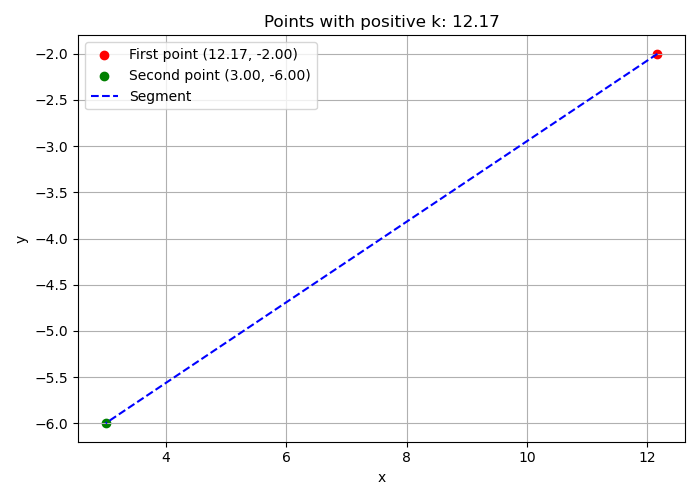
\includegraphics[width=\linewidth]{figs/points.png}
    \caption{}
\end{figure}
\end{frame}

\begin{frame}[fragile]
\frametitle{C-Code}
\begin{lstlisting}[language=C]
#include <stdio.h>
#include <math.h>

// Fills k and both point arrays.
void find_k_and_points(double *k, double pt1[2], double pt2[2]) {
    *k = 3 + sqrt(84);
    pt1[0] = *k;  pt1[1] = -2;
    pt2[0] = 3;   pt2[1] = -6;
}

int main() {
    double k, pt1[2], pt2[2];
    find_k_and_points(&k, pt1, pt2);
    printf("Positive value of k: %.6f\n", k);
    printf("First point: (%.6f, %.6f)\n", pt1[0], pt1[1]);
    printf("Second point: (%.6f, %.6f)\n", pt2[0], pt2[1]);
    return 0;
}

 \end{lstlisting}
\end{frame}

\begin{frame}[fragile]
\frametitle{Python-Code}
\begin{lstlisting}
# Code by GVV Sharma
# Modified for Problem Solution
# Released under GNU GPL
# Calculating area enclosed between curves
import ctypes
import numpy as np

# Load compiled shared library
lib = ctypes.CDLL('./code.so')

# Set function argument and return types
lib.find_k_and_points.argtypes = [
    ctypes.POINTER(ctypes.c_double),          # double *k
    np.ctypeslib.ndpointer(dtype=np.double, ndim=1, flags='C_CONTIGUOUS'), # pt1[2]

\end{lstlisting}
\end{frame}

\begin{frame}[fragile]
\frametitle{Python-Code}
\begin{lstlisting}
np.ctypeslib.ndpointer(dtype=np.double, ndim=1, flags='C_CONTIGUOUS')  # pt2[2]
]
lib.find_k_and_points.restype = None

def get_points():
    k = ctypes.c_double()
    pt1 = np.zeros(2, dtype=np.double)
    pt2 = np.zeros(2, dtype=np.double)
    lib.find_k_and_points(ctypes.byref(k), pt1, pt2)
    return k.value, pt1, pt2

\end{lstlisting}
\end{frame}

\begin{frame}[fragile]
\frametitle{Python-Code}
\begin{lstlisting}
import matplotlib.pyplot as plt
import numpy as np
from call import get_points

k, pt1, pt2 = get_points()

plt.figure(figsize=(7,5))
plt.scatter(pt1[0], pt1[1], color='red', label=f'First point ({pt1[0]:.2f}, {pt1[1]:.2f})')
plt.scatter(pt2[0], pt2[1], color='green', label=f'Second point ({pt2[0]:.2f}, {pt2[1]:.2f})')

\end{lstlisting}
\end{frame}

\begin{frame}[fragile]
\frametitle{Python-Code}
\begin{lstlisting}
plt.plot([pt1[0], pt2[0]], [pt1[1], pt2[1]], 'b--', label='Segment')
plt.title(f'Points with positive k: {k:.2f}')
plt.xlabel('x')
plt.ylabel('y')
plt.legend(loc='best')
plt.grid(True)
plt.tight_layout()
plt.show()


\end{lstlisting}
\end{frame}

\end{document}